\chapter{机器学习}
\label{chap:machinelearning}

\section{分类问题}
分类问题就是将数据以一定的分类标准分为几簇,在本节中,我们将介绍几种分类方法。
第一种分类方法是SVM(Support Vector Machine,支持向量机),是机器学习中经典的算法。
我们以简单的逻辑分类为例,如图\ref{SVM_picture}所示,我们需要找到一条直线,这样就能将所有的数据分为两类。

\begin{figure}[!ht]
    \begin{center}
    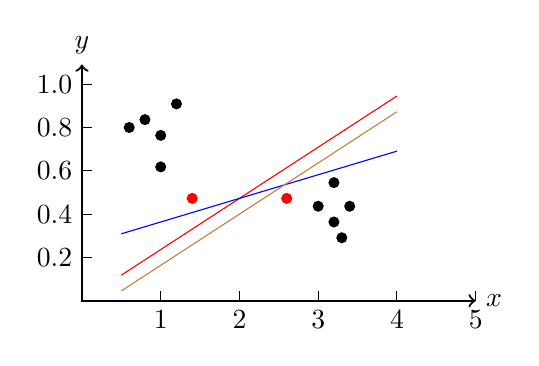
\begin{tikzpicture}
        \pgfmathsetmacro{\ticker}{0.125}
        \draw [<->,thick] (0,3) node (yaxis) [above] {$y$}
                |- (5,0) node (xaxis) [right] {$x$};
        \foreach \i/\texti  in {1,2,3,4,5} {
        \draw (1*\i,0) --(1*\i,\ticker) node[label=below:\texti]{};
        }
        \foreach \j/\textj  in {0.2,0.4,0.6,0.8,1.0} {
        \draw (0,2.75*\j) --(\ticker,2.75*\j) node[label=left:\textj]{};
        }
        \fill[black] (1,1.7) circle (2pt);
        \fill[black] (0.6,2.2) circle (2pt);
        \fill[black] (0.8,2.3) circle (2pt);
        \fill[black] (1,2.1) circle (2pt);
        \fill[black] (1.2,2.5) circle (2pt);
        \fill[red] (1.4,1.3) circle (2pt);
        
        \fill[black] (3.2,1) circle (2pt);
        \fill[black] (3,1.2) circle (2pt);
        \fill[black] (3.2,1.5) circle (2pt);
        \fill[black] (3.3,0.8) circle (2pt);
        \fill[black] (3.4,1.2) circle (2pt);
        \fill[red] (2.6,1.3) circle (2pt);
        
        \draw[color=red, domain=0.5:4]    plot (\x,{0.65 * \x}) node[right]{};
        \draw[color=blue, domain=0.5:4]    plot (\x,{0.3 * \x + 0.7}) node[right]{};
        \draw[color=brown, domain=0.5:4]  plot(\x,{0.65 * \x - 0.2}) node[right] {};
        \end{tikzpicture}
        \caption{支持向量机示意图}
        \label{SVM_picture}
    \end{center}
    \end{figure}


如果不加以限制,这样的分类直线将有无数条。
为了在众多的直线中找到最优的分类直线,我们要遵循间隔最大化原则,
即分类直线离数据越远就是最优的,因为如果不是这样,
分类直线会紧贴边界的数据;这时如果出现一个与边界数据略有不同的新数据,
就很容易被分到错误的一边。同时,过于接近分类直线的数据点不具有太大的实际意义。
想要达到分类直线离数据最远的效果,我们需要找到离分类直线最近的数据点,
用它们与直线的距离来训练神经网络。这些数据点被称为支持向量,这也是支持向量机名字的由来。

还是以图\ref{SVM_picture}为例,图中两个红色的点为支持向量,也就是离分类直线最近的两个点。
蓝线因为离两个支持向量都不是最远,所以不是最佳分类直线;棕线离上方的支持向量足够远,
然而最佳分类直线应与所有支持向量保持最远距离,
即所有支持向量离直线等距且最远,所以棕线也不符合要求。红线符合上述所有要求,
时这个数据集的最佳分类直线。

分类问题的第二种分类方法是RBM(Restricted Boltzmann Machine,受限波兹曼机)。
RBM是一种无向图模型,具有两层结构:可见层(V层),隐藏层(H层),这两层的节点相互全部连接,
但是每一层各自的神经元之间没有连接,因此被称为受限波兹曼机。波兹曼机是允许同一层神经元连接的。



\begin{figure}
    \begin{center}
    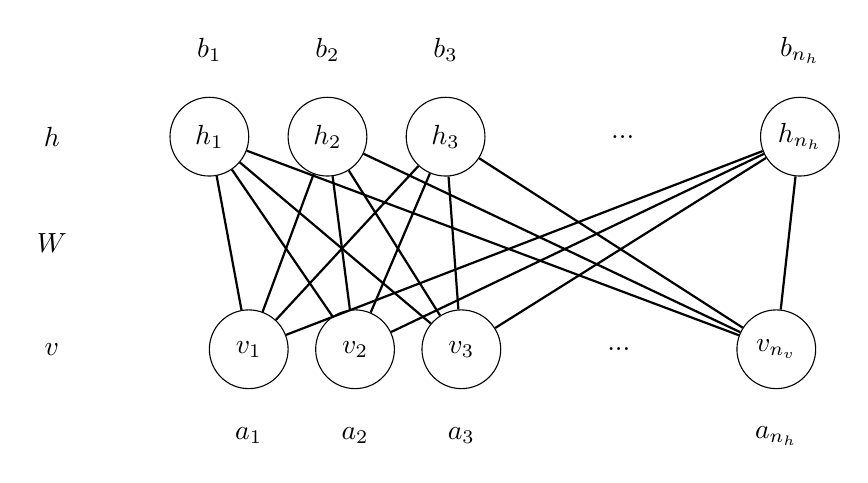
\begin{tikzpicture}
    \tikzstyle{arrow} = [thick, -, >= stealth]
    \tikzstyle{node} = [circle,  minimum width = 1cm, minimum height=1cm ,text centered, draw = black]
    \node[](H){$h$};
    \node[node, right of = H, xshift = 1cm](H1){$h_1$};
    \node[node, right of = H1, xshift = 0.5cm](H2){$h_2$};
    \node[node, right of = H2, xshift = 0.5cm](H3){$h_3$};
    \node[right of = H3, xshift = 1.25cm](...){...};
    \node[node, right of = ..., xshift = 1.25cm](Hn){$h_{n_h}$};

    \node[below of = H, yshift = -0.35cm](W){$W$};

    \node[below of = H, yshift = -1.7cm](V){$v$};
    \node[node, right of = V,xshift = 1.5cm](V1){$v_1$};
    \node[node, right of = V1, xshift = 0.35cm](V2){$v_2$};
    \node[node, right of = V2, xshift = 0.35cm](V3){$v_3$};
    \node[right of = V3, xshift = 1cm](...1){...};
    \node[node, right of = ...1, xshift = 1cm](Vn){$v_{n_v}$};
    
    \node[above of = H1, yshift = 0.1cm](b1){$b_1$};
    \node[above of = H2, yshift = 0.1cm](b2){$b_2$};
    \node[above of = H3, yshift = 0.1cm](b3){$b_3$};
    \node[above of = Hn, yshift = 0.1cm](bn){$b_{n_h}$};
    
    \node[below of = V1, yshift = -0.1cm](a1){$a_1$};
    \node[below of = V2, yshift = -0.1cm](a2){$a_2$};
    \node[below of = V3, yshift = -0.1cm](a3){$a_3$};
    \node[below of = Vn, yshift = -0.1cm](an){$a_{n_h}$};

    \draw[arrow] (H1)--(V1);
    \draw[arrow] (H1)--(V2);
    \draw[arrow] (H1)--(V3);
    \draw[arrow] (H1)--(Vn);
    \draw[arrow] (H2)--(V1);
    \draw[arrow] (H2)--(V2);
    \draw[arrow] (H2)--(V3);
    \draw[arrow] (H2)--(Vn);
    \draw[arrow] (H3)--(V1);
    \draw[arrow] (H3)--(V2);
    \draw[arrow] (H3)--(V3);
    \draw[arrow] (H3)--(Vn);
    \draw[arrow] (Hn)--(V1);
    \draw[arrow] (Hn)--(V2);
    \draw[arrow] (Hn)--(V3);
    \draw[arrow] (Hn)--(Vn);

    \end{tikzpicture}
    \caption{受限波兹曼机模型结构}
    \label{SVM_model_picture}
    \end{center}
\end{figure}


另外,受限波兹曼机是二值化的,也就是说,其神经元的输出只有两种状态:激活和未激活,
一般情况下我们分别用1和0表示。在图\ref{SVM_model_picture}所示的例子中,$n_v$和$n_h$分别表示可见层和隐藏层的神经元数目;
前面我们提到,受限波兹曼机的神经元只有激活和未激活两种状态,因此,
我们可以用向量v来表示可见层的状态向量,具体表达式为$\mathbf{v}=\left(v_{1}, v_{2}, \cdots, v_{n_{v}}\right)^{T}$,
其中$v_i$表示可见层中第i个神经元的状态。同理,
隐藏层的状态向量也可以表示为$\mathbf{h}=\left(h_{1}, h_{2}, \cdots, h_{n_{h}}\right)^{T}$,
其中$h_i$表示可见层中第i个神经元的状态。
可见层的偏置向量用a来表示,具体表达式为$\mathbf{a}=\left(a_{1}, a_{2}, \cdots, a_{n_{v}}\right)^{T}$,
同样的,隐藏层的偏置向量为b,表达式为$\mathbf{b}=\left(b_{1}, b_{2}, \cdots, b_{n_{h}}\right)^{T}$。


最后,连接隐藏层和可见层的权值矩阵用$w$来表示,表达式为$W=\left(w_{i, j}\right)$,$w_{i,j}$代表
隐藏层中第i个神经元与可见层中第j个神经元之间的连接权重。


有了这些前置参数,我们便可以探索受限波兹曼机的更多特性和用途。
受限波兹曼机是一个能量模型(Energy Based Model, EBM),是由物理学能量模型演变而来;
能量模型需要先定义一个合适的能量函数,
然后基于这个能量函数得到变量的概率分布,最后基于概率分布去求解一个目标函数。
受限波兹曼机的能量函数定义为:

\begin{equation}
E_{\theta}(\mathbf{v}, \mathbf{h})=-\sum_{i=1}^{n_{v}} a_{i} v_{i}-\sum_{j=1}^{n_{h}} b_{j} h_{j}-\sum_{i=1}^{n_{v}} \sum_{j=1}^{n_{h}} h_{j} w_{j, i} v_{i}
\end{equation}


如果写成矩阵的形式,则可改写为

\begin{equation}
E_{\theta}(\mathbf{v}, \mathbf{h})=-\mathbf{a}^{T} \mathbf{v}-\mathbf{b}^{T} \mathbf{h}-\mathbf{h}^{T} W \mathbf{v}
\end{equation}

相比于波兹曼机(BM),受限波兹曼机(RBM)因其具有快速学习的特点而被广泛地使用。
与此同时,RBM在分类,回归和图像特征提取上也得到了广泛的应用。



\section{线性回归}
线性回归是机器学习解决预测问题的重要途径之一。
在进行线性回归算法时,我们通常会指定一个数据集,其中包括了正确答案。
线性回归算法会根据给出的数据集去拟合一个函数,使之尽量符合所给出的数据集,
同时达到预测更多正确答案的效果。(如图\ref{Linear_picture}所示)
这种模式类似于老师给定多个参数和结果,让学生自己寻找函数并且不断地自我修正;
同时老师也会监督并量化期望与实际输出间的误差。
因此,线性回归算法也被称为监督学习。

\begin{figure}[!hb]
\begin{center}
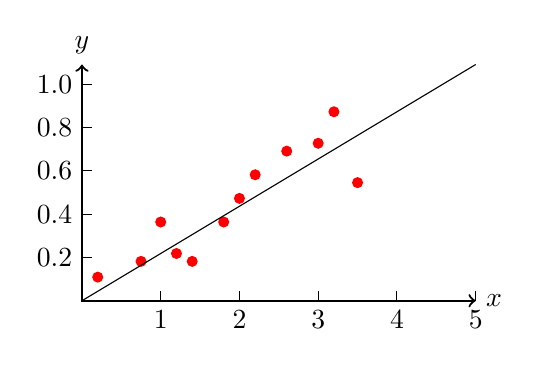
\begin{tikzpicture}
    \pgfmathsetmacro{\ticker}{0.125}
    \draw [<->,thick] (0,3) node (yaxis) [above] {$y$}
            |- (5,0) node (xaxis) [right] {$x$};
    \foreach \i/\texti  in {1,2,3,4,5} {
    \draw (1*\i,0) --(1*\i,\ticker) node[label=below:\texti]{};
    }
    \foreach \j/\textj  in {0.2,0.4,0.6,0.8,1.0} {
    \draw (0,2.75*\j) --(\ticker,2.75*\j) node[label=left:\textj]{};
    }
    \
    \fill[red] (0.2,0.3) circle (2pt);
    \fill[red] (0.75,0.5) circle (2pt);
    \fill[red] (1,1) circle (2pt);
    \fill[red] (1.2,0.6) circle (2pt);
    \fill[red] (1.4,0.5) circle (2pt);
    \fill[red] (1.8,1) circle (2pt);
    \fill[red] (2.0,1.3) circle (2pt);
    \fill[red] (2.2,1.6) circle (2pt);
    \fill[red] (2.6,1.9) circle (2pt);
    \fill[red] (3,2.0) circle (2pt);
    \fill[red] (3.2,2.4) circle (2pt);
    \fill[red] (3.5,1.5) circle (2pt);
    \draw (0,0) -- (5,3) node [] {};
    \end{tikzpicture}
    \caption{根据所给的数据集拟合函数,并根据此函数预测将来的数值}
    \label{Linear_picture}
\end{center}
\end{figure}


如图\ref{Linear_picture}所示,自变量x会与要预测的目标变量y建立一个函数关系。
为了使结果更精确,我们可以指定特定的模型,决定是使用一次函数还是二次函数来更好地贴合数据集,
从而达到更好的预测效果。

在DL4J中,线性回归算法主要有三个部分组成,模型的建立,过程的监听和数据集的构造。
建立模型需要一些超参数。在下面的代码块中指定了一些超参数:第一是随机种子,
由于每次进行神经网络训练时,函数的偏置和权重都是随机的,
我们需要用种子来确保初始情况大致一致,使结果具有可复现性。
第二是OptimizationAlgorithm 和updater,代表了模型的优化算法,
分别决定了学习的方向和学习率的大小。第三是对模型权重的初始化。
第四是对神经元的设置,第六是设置是否进行反向传播。

\begin{figure}[!ht]
\begin{lstlisting}[language=Java]
 MultiLayerConfiguration conf = new NeuralNetConfiguration.Builder()
                .seed(seed)
                .optimizationAlgo(OptimizationAlgorithm.STOCHASTIC_
                GRADIENT_DESCENT)
                .weightInit(WeightInit.XAVIER)
                .updater(new Sgd(learningRate))
                .layer(0, new OutputLayer.Builder(LossFunctions.LossFunction.MSE)
                .backprop(true)
                .build
\end{lstlisting}
\end{figure}

在进行训练的同时我们也要对模型进行监听,
主要用于对函数的损失函数进行监听,从而更好地对算法进行改进。

最后是数据集的构造。我们说过线性回归的数据集包括数据和结果两个部分。
在这里,我们把自变量x称为特征,因变量y称为标签,
首先先创建两个长度为样本数量的数组,分别代表输入和输出数据的数组;
接着根据特征的值随机生成输入和输出的数,最后将其包装成一个类返回给模型,
代码如图\ref{statics_set_creation}所示。

\begin{figure}[!ht]
\begin{lstlisting}[language=Java]
  private static DataSetIterator getTrainingData(int batchSize, Random rand) {
        double [] output = new double[SampleNum];
        double [] input = new double[SampleNum];
        for (int i= 0; i< SampleNum; i++) {
            input[i] = MIN_RANGE + (MAX_RANGE - MIN_RANGE) * rand.nextDouble();
            output[i] = 0.5 * input[i] + 0.1;
        }
        INDArray inputNDArray = Nd4j.create(input, new int[]{nSamples,1});

        INDArray outPut = Nd4j.create(output, new int[]{nSamples, 1});
        DataSet dataSet = new DataSet(inputNDArray, outPut);
        List<DataSet> listDs = dataSet.asList();
        return new ListDataSetIterator(listDs,batchSize);
    }
\end{lstlisting}
\caption{数据集的构造:包括特征和标签}
\label{statics_set_creation}
\end{figure}


当然,这里的线性回归只含有一个自变量和一个因变量,因此被称为一次线性回归或单变量线性回归。
这种模型比较简单,用二维的xy坐标轴即可表示出来。
在实际的操作中还会遇到还有多变量线性回归,在面对更多维度的参数能更好地进行处理。


\subsection{过拟合}
对于机器学习来说,过拟合是一个十分常见的问题。
过拟合具体是指经过机器学习所获得的权重参数,可以拟合训练数据,
却在面对不包含在训练数据中的实际数据时,不能很好的拟合他们。
机器学习的目的就是获得一个更加抽象,以及泛化的模型。
即使是面对未包含在训练数据中的数据,我们也希望能获得较好的拟合结果。
所以我们需要通过一定的方法来抑制过拟合。

过拟合产生的原因,主要有两点:
1.模型具有大量的参数,表现力强
2.训练数据的数量很少


\begin{figure}[!ht]
\begin{center}
\begin{tikzpicture}
    \pgfmathsetmacro{\ticker}{0.125}
    \draw [<->,thick] (-0.5,5) node (yaxis) [above] {$x_2$}
            |- (4,0.4) node (xaxis) [right] {$x_1$};
    \
     \draw[dashed](0,0.7)--(0.2,1.3);
     \draw[dashed](0.2,1.3)--(0.5,1.7);
     \draw[dashed](0.5,1.7)--(0.7,2);
     \draw[dashed](0.7,2)--(0.8,3.2);
     \draw[dashed](0.8,3.2)--(1,3.8);
     \draw[dashed](1,3.8)--(1.3,4.2);
     \draw[dashed](1.3,4.2)--(1.4,4.5);
     \draw[dashed](1.4,4.5)--(1.6,4.6);
     \draw[dashed](1.6,4.6)--(1.8,4.8);
     \draw[dashed](1.8,4.8)--(1.9,4.9);
     \draw[dashed](1.9,4.9)--(2.0,4.92);
     \draw[dashed](2.0,4.92)--(2.1,4.93);
     \draw[dashed](2.1,4.93)--(2.3,4.94);
     \draw[dashed](2.3,4.94)--(2.5,4.95);
     \draw[dashed](2.5,4.95)--(2.8,4.97);
     \draw[dashed](2.8,4.97)--(3,5);
     \draw[gray](0,0.7)--(0.2,1.2);
     \draw[gray](0.2,1.2)--(0.5,1.3);
     \draw[gray](0.5,1.3)--(0.7,1.5);
     \draw[gray](0.7,1.5)--(0.8,2.2);
     \draw[gray](0.8,2.2)--(1,2.8);
     \draw[gray](1,2.8)--(1.3,3);
     \draw[gray](1.3,3)--(1.4,3.2);
     \draw[gray](1.4,3.2)--(1.6,3.3);
     \draw[gray](1.6,3.3)--(1.8,3.4);
     \draw[gray](1.8,3.4)--(1.9,3.42);
     \draw[gray](1.9,3.42)--(2.2,3.43);
     \draw[gray](2.2,3.43)--(2.5,3.46);
     \draw[gray](2.5,3.46)--(2.8,3.48);
     \draw[gray](2.8,3.48)--(3,3.5);
\end{tikzpicture}
\caption{过拟合情况}
\label{over_fitting}
\end{center}
\end{figure}

如图\ref{over_fitting}所示,对于训练用数据来说,大约100个epoch之后,精度便可以达到接近100\%。
但是,对于测试用数据来说,识别精度确只能达到70\%左右,这并非我们所想要的结果。
从上面的分析中可知,模型对训练时没有使用的数据拟合得并不好。

\subsection{正则化}
过拟合作为机器学习中一种常见的问题,自然也有解决的方法。
基于本书主要介绍关于入门方面的知识,在此便不深入介绍。
仅简单介绍一下权值衰减这一方法。

权值衰减是一种常见的用来抑制过拟合的方法。其通过在学习过程在中
对大的权重进行一定比例的惩罚,从而达到过拟合的目的。过拟合往往就是因为
权重参数取值过大才发生的。因此权值衰减不失为一种简单而有效的办法。

实现权值衰减具体方法是为损失函数加上权重的平方范数(L2范数)。
机器学习的目的是减少损失函数的值,使用权值衰减后,
便可以对变大的权重进行惩罚,从而达到抑制的作用。
具体来说,如果将权重记为$\boldsymbol{W}$,L2范数的值便是$\frac{1}{2}\lambda\boldsymbol{W}^2$。
权值衰减便是将L2范数加到损失函数中。在L2范数中,$\lambda$是控制正则化程度的参数。
$\lambda$越大,对数值较大的权重施加的惩罚也就越重。
下面我们用图片来具体解释:

\begin{figure}[!ht]
    \begin{center}
    \begin{tikzpicture}
        \pgfmathsetmacro{\ticker}{0.125}
        \draw [<->,thick] (-0.5,5) node (yaxis) [above] {$x_2$}
                |- (4,0.4) node (xaxis) [right] {$x_1$};
        \
         \draw[dashed](0,0.7)--(0.2,1.3);
         \draw[dashed](0.2,1.3)--(0.5,1.7);
         \draw[dashed](0.5,1.7)--(0.7,2);
         \draw[dashed](0.7,2)--(0.8,3.2);
         \draw[dashed](0.8,3.2)--(1,3.6);
         \draw[dashed](1,3.6)--(1.3,3.8);
         \draw[dashed](1.3,3.8)--(1.4,4);
         \draw[dashed](1.4,4)--(1.6,4.1);
         \draw[dashed](1.6,4.1)--(1.8,4.3);
         \draw[dashed](1.8,4.3)--(1.9,4.4);
         \draw[dashed](1.9,4.4)--(2.0,4.42);
         \draw[dashed](2.0,4.42)--(2.1,4.47);
         \draw[dashed](2.1,4.47)--(2.3,4.43);
         \draw[dashed](2.3,4.43)--(2.5,4.49);
         \draw[dashed](2.5,4.49)--(2.8,4.45);
         \draw[dashed](2.8,4.45)--(3,4.5);
         \draw[gray](0,0.7)--(0.2,1.2);
         \draw[gray](0.2,1.2)--(0.5,1.3);
         \draw[gray](0.5,1.3)--(0.7,1.5);
         \draw[gray](0.7,1.5)--(0.8,2.2);
         \draw[gray](0.8,2.2)--(1,2.8);
         \draw[gray](1,2.8)--(1.3,3);
         \draw[gray](1.3,3)--(1.4,3.2);
         \draw[gray](1.4,3.2)--(1.6,3.3);
         \draw[gray](1.6,3.3)--(1.8,3.4);
         \draw[gray](1.8,3.4)--(1.9,3.42);
         \draw[gray](1.9,3.42)--(2.2,3.43);
         \draw[gray](2.2,3.43)--(2.5,3.46);
         \draw[gray](2.5,3.46)--(2.8,3.48);
         \draw[gray](2.8,3.48)--(3,3.5);
    \end{tikzpicture}
    \caption{权值衰减方法}
    \end{center}
    \end{figure}

如上图所示,测试数据的识别精度没有太大变化。但训练数据和测试数据的识别精度之间的差距
明显缩小了。这证明,过拟合收到了抑制,而训练数据和测试数据的整体识别精度的增加需要依靠其他的
方法,并非权值衰减的作用范围。

\section{逻辑回归}
逻辑回归与线性回归相似,同样用于处理数据的分类问题。
他们的不同之处在于逻辑回归的数据集中只包含数据,神经网络会自我学习,
自行生成一套数据结构模式。在这种模式中,我们只需要提供数据,
不需要提供数据集地的正确答案,其余部分均由神经网络完成对数据的分类。
因此,逻辑回归也被称为无监督学习。

在下图的例子中,我们给出一个数据集(如图\ref{Logic_picture})。
模型并不知道这些数据的意义和用途,只会尝试着找出其中潜藏的数据结构。
在这个例子中,逻辑回归算法会判定这个数据集从属于两个数据簇$a$,$b$,
从而完成数据分类的任务。
\vspace{5pt}

    \begin{figure}[!hb]
    \begin{center}
    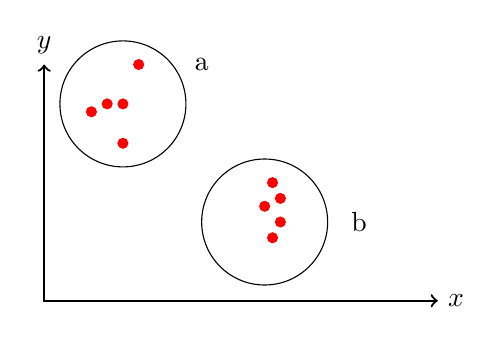
\begin{tikzpicture}
    \draw [<->,thick] (0,3) node (yaxis) [above] {$y$}
        |- (5,0) node (xaxis) [right] {$x$};
    \fill[red] (1,2) circle (2pt);
    \fill[red] (0.6,2.4) circle (2pt);
    \fill[red] (0.8,2.5) circle (2pt);
    \fill[red] (1,2.5) circle (2pt);
    \fill[red] (1.2,3) circle (2pt);
    \node at (2,3) {a};
    \draw  (1,2.5) ellipse (0.8 and 0.8);
    \fill[red] (3,1) circle (2pt);
    \fill[red] (2.8,1.2) circle (2pt);
    \fill[red] (2.9,1.5) circle (2pt);
    \fill[red] (2.9,0.8) circle (2pt);
    \fill[red] (3,1.3) circle (2pt);
    \draw  (2.8,1) ellipse (0.8 and 0.8);
    \node at (4,1) {b};
    \end{tikzpicture}
    \caption{逻辑回归注重数据的分类}
    \label{Logic_picture}
    \end{center}
    \end{figure}


在DL4J中,逻辑回归与线性回归配置类似,主要区别在于神经网络的最后一层输出层:
在线性回归中,最后一个隐藏层是Activation.IDENTITY,即不对数据作处理。
而逻辑回归的最后一层为Activation.SOFTMAX,指定了对当前数据进行分类任务。
代码如下:

\begin{figure}[!hb]
\begin{lstlisting}[language=Java]
        MultiLayerConfiguration conf = new NeuralNetConfiguration.Builder()
        .seed(seed)
        .updater(new Nesterovs(learningRate, 0.9))
        .layer(0, new OutputLayer.Builder(LossFunction.NEGATIVELOGLIKELIHOOD)
                .weightInit(WeightInit.XAVIER)
                .activation(Activation.SOFTMAX)
                .build())
        .build();
\end{lstlisting}
\end{figure}


\section{正向传播}
正向传播也叫前向传播,是指数据从输入层到隐藏层,再到输出层的单向过程。
数据会从输入层输入,经过隐藏层的一层层地变换,最终得出结果数据。
如图\ref{three_layers_picture}是一个典型的三层神经网络,
我们便以此为例解释正向传播。

\begin{figure}[!ht]
    \begin{center}
    \begin{tikzpicture}
    \tikzstyle{arrow} = [thick, ->, >= stealth]
    \tikzstyle{node} = [circle,  minimum width = 1cm, minimum height=1cm ,text centered, draw = black]
    \node[node](I1){$I_1$};
    \node[node, below of = I1, yshift = -1cm](I2){$I_2$};
    \node[node, below of = I2, yshift = -1cm](I3){$I_3$};
    \node[node, right of = I1, xshift = 1.5cm](H1){$H_1$};
    \node[node, right of = I2, xshift = 1.5cm](H2){$H_2$};
    \node[node, right of = I3, xshift = 1.5cm](H3){+1};
    \node[node, right of = H2, xshift = 1.5cm](O1){$O_1$};
    \node[below, below of = I3, yshift = -0.5cm](text1){输入层};
    \node[below, below of = H3, yshift = -0.5cm](text2){隐藏层};
    \node[below, right of = text2, xshift = 1.5cm](text3){输出层};

    \draw[arrow] (I1)--(H1);
    \draw[arrow] (I1)--(H2);
    \draw[arrow] (I2)--(H1);
    \draw[arrow] (I2)--(H2);
    \draw[arrow] (I3)--(H1);
    \draw[arrow] (I3)--(H2);
    \draw[arrow] (H1)--(O1);
    \draw[arrow] (H2)--(O1);
    \draw[arrow] (H3)--(O1);
    \end{tikzpicture}
    \caption{经典的三层神经网络}
    \label{three_layers_picture}
    \end{center}
\end{figure}

隐藏层$H_1$的值由输入层的值和权重所决定,
$W_{(1,1)}$,$W_{(2,1)}$,$W_{(3,1)}$分别代表输入数据$I_1$,$I_2$,$I_3$
对于隐藏层$H_1$的权重。公式如下:

\begin{equation*}
    H_1=I_1W_{(1,1)}+I_2W_{(2,1)}+I_3W_{(3,1)}
\label{Propgate_equation}
\end{equation*}


同理,$H_2$也可表达为相似的公式。经由隐藏层激活函数计算后得到该层的激活值。
同时,输出层的值由隐藏层的值和权值决定,$W_1$,$W_2$分别代表各个隐藏层数据对于
输出层的权重。$b_1$表示偏置,公式如下:

\begin{equation*}
    O_1=H_1W_1+H_2W_2+b_1
    \label{Propgate_output_equation}
\end{equation*}

这样一个由输入层至隐藏层,再由隐藏层至输出层的过程就被称为正向传播。
如图\ref{three_layers_picture}所示,只含有正向传播的神经网络可以用一个有向无环图来表示。
只含有正向传播的神经网络被称为前馈神经网络,
是现今发展较为成熟的一种神经网络。


\section{反向传播}
在正向传播中,神经网络中的数据单向向前传播;因此,我们无法准确知道每一步造成的误差大小,
也无法根据误差对神经网络进行调整更新;反向传播就提供了另一种途径来量化误差并更新权值。
反向传播用于将代价函数最小化,将每一层的误差反向传播给上一层,
由此将误差最小化,如图\ref{back_propagate_picture}。


\begin{figure}[!ht]
    \begin{center}
    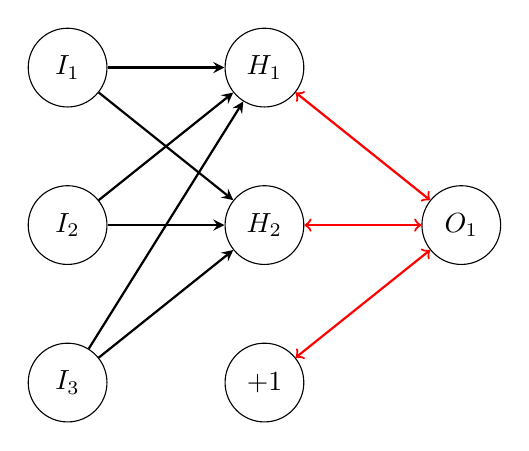
\begin{tikzpicture}
    \tikzstyle{arrow} = [thick, ->, >= stealth]
    \tikzstyle{arrowred} = [thick,<->,red]
    \tikzstyle{node} = [circle,  minimum width = 1cm, minimum height=1cm ,text centered, draw = black]
    \node[node](I1){$I_1$};
    \node[node, below of = I1, yshift = -1cm](I2){$I_2$};
    \node[node, below of = I2, yshift = -1cm](I3){$I_3$};
    \node[node, right of = I1, xshift = 1.5cm](H1){$H_1$};
    \node[node, right of = I2, xshift = 1.5cm](H2){$H_2$};
    \node[node, right of = I3, xshift = 1.5cm](H3){+1};
    \node[node, right of = H2, xshift = 1.5cm](O1){$O_1$};
    \draw[arrow] (I1)--(H1);
    \draw[arrow] (I1)--(H2);
    \draw[arrow] (I2)--(H1);
    \draw[arrow] (I2)--(H2);
    \draw[arrow] (I3)--(H1);
    \draw[arrow] (I3)--(H2);
    \draw[arrowred] (H2)--(O1);
    \draw[arrowred] (H3)--(O1);
    \draw[arrowred] (O1)--(H1);
    \end{tikzpicture}
    \caption{具有反向传播的神经网络}
    \label{back_propagate_picture}
    \end{center}
\end{figure}


为了计算每一层神经元所产生的误差,我们引入$\delta_{j}^{(l)}$,
代表第l层的第j个节点所产生的误差。
由此可得最后一层输出层的误差公式为$\delta_{j}^{(3)}=a_{j}^{(3)}-y_{j}$,其中$a_{j}^{(3)}$
代表神经网络计算出的值,而$y_{j}$代表数据对应的真实值。

误差向前一层传播时,公式需更改为
$\delta^{(2)}=(\Theta^{(2)})^{T}\delta^{(3)}*g'(z^{(2)})$,$(\Theta^{(n)})^T$代表
第n层代价函数的转置,$z^{(n)}$等于$\Theta^{(n-1)} a^{(n-1)}$,最后
$g(z)$代表该层的激活函数。依据这个公式,我们就而可以将误差逐层上传,并实现对神经网络
参数的修改。

反向传播实际上与正向传播很相似。他们的计算方法类似,区别在于正向传播是从前向后计算,
而反向传播是从后向前计算。其实,$\delta_{j}^{(l)}$即是
该层代价函数关于该层对应的所有输入单元加权和的偏导。以图\ref{back_propagate_picture}为例,$\delta_{1}^{(3)}$可表达为
$\delta_{1}^{(3)}=\frac{\partial}{\partial z_{1}^{(3)}} \operatorname{cost}(\mathrm{i})$,
其中$cost(i)$代表该层的代价函数,
$z_{1}^{(3)}$等于$a_{1}^{(2)}*W_{(1,2)}+a_{2}^{(2)}*W_{(2,2)}$。
$\delta_{j}^{(l)}$衡量了神经网络计算中的中间值,代表了神经网络权重改变的程度大小,
使我们对整个网络有更深入的了解。

反向传播只是正向传播的逆向过程。我们还是以图\ref{back_propagate_picture}为例,
由上可知$\delta_{1}^{(3)}=a_{1}^{(3)}-y_{1}$,而逆向到$\delta_{2}^{(2)}$的算式
可表达为$\delta_{2}^{(2)}=(W_{(2,2)})^{-1}*\delta_{1}^{(3)}$。这样的逆过程与
正向传播的计算过程区别不大;所以说,反向传播与正向传播在形式和计算方法上都很相似。

反向传播广泛地应用于循环神经网络,例如机器翻译、语言理解等前沿应用。
这种结构的网络往往存在记忆单元和注意力机制,要求复杂的求导计算,
例如Google语音助手的上下文理解功能。反向传播促进了记忆神经网络的发展,
目前正在探索和发展中。



\section{全连接网络}
全连接层网络(MLP,Multilayer Perceptron)又叫多层感知机,
特点是上一层的所有神经元都与下一层的所有神经元相连接,因此又叫全连接层。
如图\ref{three_layers_picture}就是一个简单的全连接层,最底层是输入层,中间是隐藏层,最后是输出层。
在计算第n层的某个节点的时候,输入的参数是第n-1层的所有节点的加权。

从图\ref{multilayer_perceptron}可以看出,全连接网络的所有参数就是各个层的权重和偏置。
确定并最优化这些参数就是一个最优化的问题,最简单的就是利用梯度下降(SGD),
首先随机初始化所有参数,然后进行迭代训练,不断地更新梯度和参数,
直到满足某个条件为止。全连接网络应用广泛,例如MNIST手写数字识别等。

\begin{figure}[!ht]
    \begin{center}
    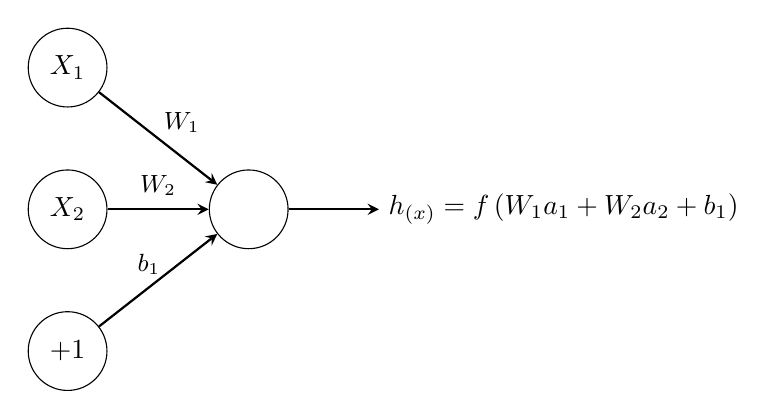
\begin{tikzpicture}
    \tikzstyle{arrow} = [thick, ->, >= stealth]
    \tikzstyle{node} = [circle,  minimum width = 1cm, minimum height=1cm ,text centered, draw = black]
    \node[node](X1){$X_1$};
    \node[node, below of = X1, yshift = -0.8cm](X2){$X_2$};
    \node[node, below of = X2, yshift = -0.8cm](+1){+1};
    \node[node, right of = X2, xshift = 1.3cm](Output){};
    \node[right of = Output, xshift = 3cm](Output1){$h_{(x)}=f\left(W_1 a_1+W_2 a_2+b_1\right)$};

    \draw[arrow](X1)--(Output);
    \draw[arrow](X2)--(Output);
    \draw[arrow](+1)--(Output);
    \draw[arrow](Output)--(Output1);

    \coordinate[label = left:{\small $W_1$}]() at(1.8, -0.7);
    \coordinate[label = left:{\small $W_2$}]() at(1.5, -1.5);
    \coordinate[label = left:{\small $b_1$}]() at(1.3, -2.5);

    \end{tikzpicture}
    \caption{全连接层中的一个节点}
    \label{multilayer_perceptron}
    \end{center}
\end{figure}



